\documentclass[12pt]{report}

% Packages
\usepackage{setspace}
\usepackage{amsmath, amssymb}
\usepackage{lineno} % for line numbering
\usepackage{graphicx}
\usepackage{geometry}
\usepackage{titlesec}
\usepackage{tabularx}
\usepackage{xcolor}
\usepackage{array}
\usepackage{booktabs}
\usepackage{natbib}
\usepackage{hyperref}

\hypersetup{
  colorlinks=false,    % Disable colored links
  pdfborder={0 0 0}    % Remove border boxes around links
}

\usepackage{multirow}
\titlespacing*{\chapter}{0pt}{0pt}{0pt}
\graphicspath{{./figures/}}

% Figure caption formatting 
\usepackage{caption}
\captionsetup{
    font={small, stretch=0.9},
    skip=5pt,
    justification=justified,
    singlelinecheck=false,
}

% Page formatting
\geometry{a4paper, left=1.5in, right=1in, top=2in, bottom=1in}
\onehalfspacing

% Title Page Command
\newcommand{\TitlePage}{
    \begin{titlepage}
        \centering
        {\large \textsc{[Thesis Title]} \\[0.4cm]}
        \vspace{2cm}
        \textit{by}\\[0.5cm]
        \textsc{[Author Name]}\\[1.5cm]
        {A Dissertation Submitted to}\\[0.5cm]
        {the Graduate Faculty of [Institution Name]}\\[1.5cm]
        {in partial fulfillment of the requirements}\\
        {for the degree of}\\[0.5cm]
        {[Degree Title]}\\[1.5cm]
        \vfill
        {[Location]}\\
        \today\\
        \thispagestyle{empty}
    \end{titlepage}
}

\begin{document}

% --------------------
%  Front matter numbering (i, ii, iii, ...)
% --------------------
% Title Page
\TitlePage

\clearpage
\pagenumbering{roman}
\setcounter{page}{2} 

%% COPYRIGHT PAGE
\newpage
\vfill
\begin{center}
    \copyright{}
    \the\year\ [Author Name]
\end{center}

% Approval Page
\newpage
This dissertation, submitted by [Author Name] in partial fulfillment of the requirements for the degree of [Degree Title] from [Institution Name], has been reviewed and approved by the Faculty Advisory Committee.\\[1cm]
\begin{flushright}
\rule{6cm}{0.4pt} \\[0.5cm]
[Chairperson Name]\\[0.5cm]
\rule{6cm}{0.4pt} \\[0.5cm]
[Committee Member Name]\\[0.5cm]
\rule{6cm}{0.4pt} \\[0.5cm]
[Committee Member Name]\\[0.5cm]
\rule{6cm}{0.4pt} \\[0.5cm]
[Member at Large]\\[0.5cm]
\end{flushright}

This dissertation is hereby approved as satisfying the requirements of [Institution Name]'s School of Graduate Studies.

\begin{flushleft}
\rule{6cm}{0.4pt}\\[0.5cm]
[Dean Name]\\
Dean, School of Graduate Studies\\[0.5cm]
\rule{6cm}{0.4pt}\\[0.5cm]
[Date]\\
\end{flushleft}

% Permission Page
\newpage
\begin{center}
    \textsc{\Large Permission}\\[1.5cm]
\end{center}
\vspace*{0.1in}
\begin{tabular}{@{}p{1in}p{\dimexpr\linewidth-1.5in\relax}@{}}
Title & {[Thesis Title]}\\[1.0cm]
Department & [Department Name] \\[0.5cm]
Degree & [Degree Title] \\[0.5cm]
\end{tabular}
\par

By submitting this dissertation as partial fulfillment of the requirements for a graduate degree at [Institution Name], I grant permission for its inclusion in the University library and for its inspection by interested scholars. Extensive copying for scholarly purposes may be authorized by the supervising professor or, if necessary, by the department chair or dean. Financial use of any portion of this work is prohibited without written permission, and proper acknowledgment must be provided in any derivative scholarly use.

\vspace{1in}
\begin{flushright}
    [Author Name]\\
    \today \\
\end{flushright}

% Acknowledgements Page
\newpage
\begin{center}
    \textsc{\Large Acknowledgements}\\[1.5cm]
    \begin{quote}
        [Express gratitude to advisors, committee members, colleagues, and family. Acknowledge contributions that were instrumental to the completion of this work.]
    \end{quote}
\end{center}

% Table of Contents, List of Figures, List of Tables
\newpage
\tableofcontents
\listoffigures
\addcontentsline{toc}{chapter}{List of Figures}
\listoftables
\addcontentsline{toc}{chapter}{List of Tables}

% Abstract
\newpage
\begin{center}
    \textsc{\Large Abstract}\\[1.5cm]
    \addcontentsline{toc}{chapter}{Abstract}
\end{center}
[Provide a concise summary of the research objectives, methodology, principal findings, and conclusions.]

% --------------------
%  Switch to Arabic numbering (1, 2, 3, ...)
% --------------------
\clearpage
\pagenumbering{arabic}

\chapter{Introduction}
\section{Introduction}

I am Albert Einstein

\begin{figure}[h!]
    \centering
    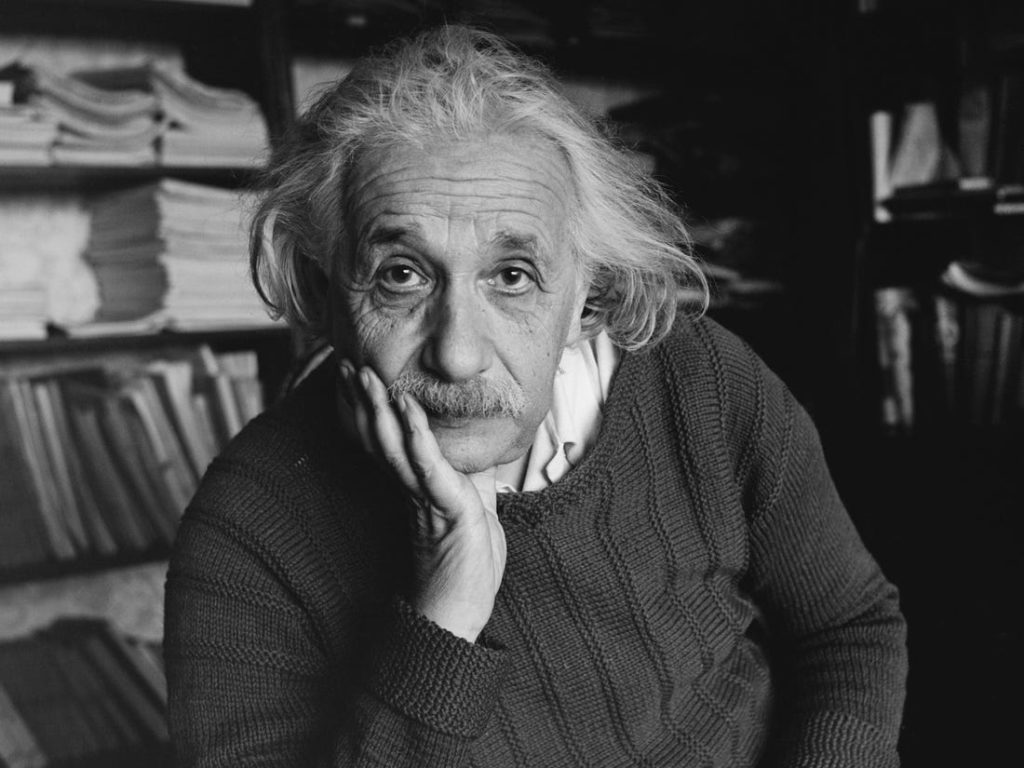
\includegraphics[width=0.8\textwidth]{einstein.jpg}
    \caption{Albert Einstein}
    \label{fig:einstein}
\end{figure}

here is einstein's paper \cite{Einstein1935}

\chapter{Literature Review}
%\input{chapter2}

\chapter{Methodology}
%\section{Introduction}

I am Albert Einstein

\begin{figure}[h!]
    \centering
    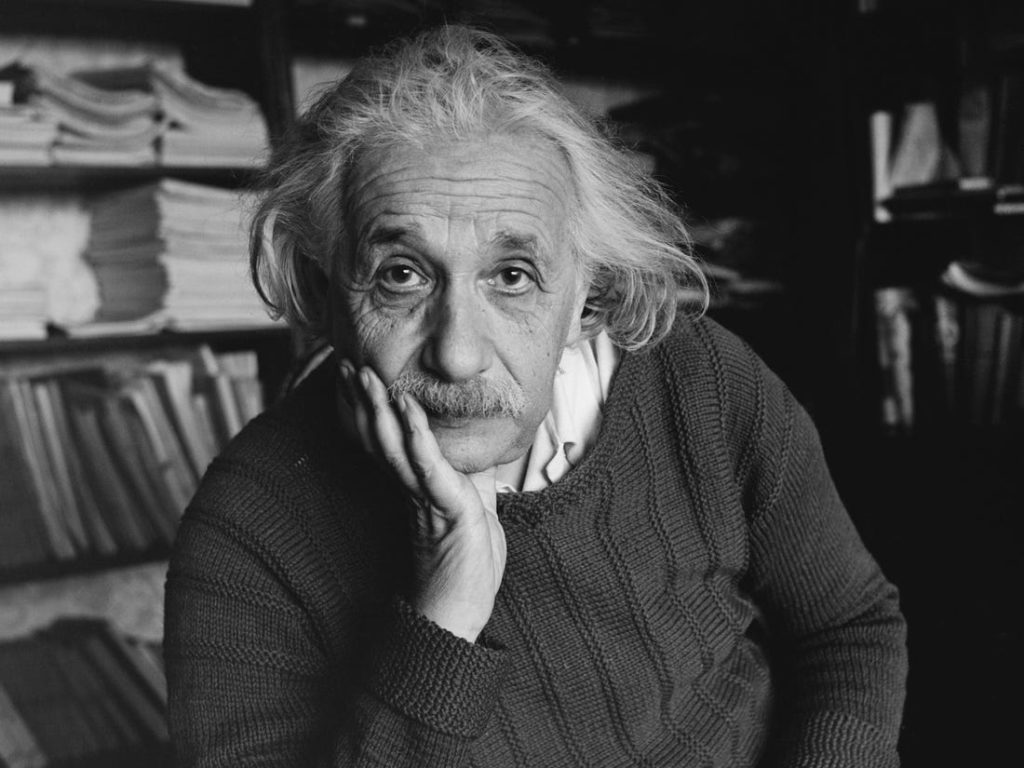
\includegraphics[width=0.8\textwidth]{einstein.jpg}
    \caption{Albert Einstein}
    \label{fig:einstein}
\end{figure}

here is einstein's paper \cite{Einstein1935}

\chapter{Results}
%\input{chapter3}

\chapter{Discussion}
%\input{chapter4}

\chapter{Conclusion}
%\input{chapter5}

% Bibliography
\newpage
\bibliographystyle{plain}
\bibliography{references}

\end{document}
